
\chapter{Discussion}
\label{chap8}
This chapter will evaluate how the implemented algorithms work, the shortcomings and
possible solutions to problems. 

\section{How did it perform?}
How the system preformed are outlined in this section. Starting off with the
\emph{SwissRanger 3000} Time-of-Flight camera.

\subsection{MESA SwissRanger 3000}
To start off, the output from the camera were applied directly into matlab. Default
integration time were used, and the intensity- and range images where captured as is from
the camera electronics.

The default readout from the ToF camera were not that affected by the difficulties
described in Chapter \ref{chap2}, but the individual range values where dominated by normal
distributed measurement errors. This where removed by averaging the images over a number
of successive images. This reduced the response time of the sensor and therefor the
refreshment time, but this will most probably not be a case in this application, since the
velocities included are not of the greatest magnitudes. 

Figure \ref{chap8:fig-typical-tof-image} shows a typical range image, and the
corresponding intensity image. 
\begin{figure}[htbp]
    \centering
    %\includegraphics[width=0.8\textwidth]{pics/tof-imagery}
    \caption{Typical range image of the pipe}
    \label{chap8:fig-typical-tof-image}
\end{figure}

When objects came too close to the sensor, it looked like the sensor went berserk. This
was because the intensity values became so large, and they dominated the picture
completely. The solution to this were to filter the range image based on the intensity
value of that pixel. An example of this can be seen in Figure
\ref{chap8:fig-tof-imagery-intensity-filtered}
\begin{figure}[htbp]
    \centering
    %\includegraphics[width=0.45\textwidth]{pics/tof-intensity-unfilterd}
    %\includegraphics[width=0.45\textwdith]{pics/tof-intensity-filtered}
    \caption{The unfiltered and filtered point clouds}
    \label{chap8:fig-tof-imagery-intensity-filtered}
\end{figure}



\subsection{Minoru 3D webcamera}
The stereo camera rig which is used in the project is a cheap mass produced stereo
webcamera. As seen from the calibration in Chapter \ref{chap3} the two different cameras have substantial
distortion, both tangential due to misaligned CCD chip, and radial due to cheap optics.
Unfortunately, the CCD chips are horizontally aligned right, while in the vertical
direction they are aligned in a divergent way. This will limit the field-of-view of the
camera. The principal axes of the two cameras are unaligned horizontally, which will
further limit the field-of-view. See figures \ref{chap2:fig-tang-dist},
\ref{chap3:fig-comp-lensdist} and \ref{chap8:fig-rad-dist}.
\begin{figure}[htbp]
    \centering
    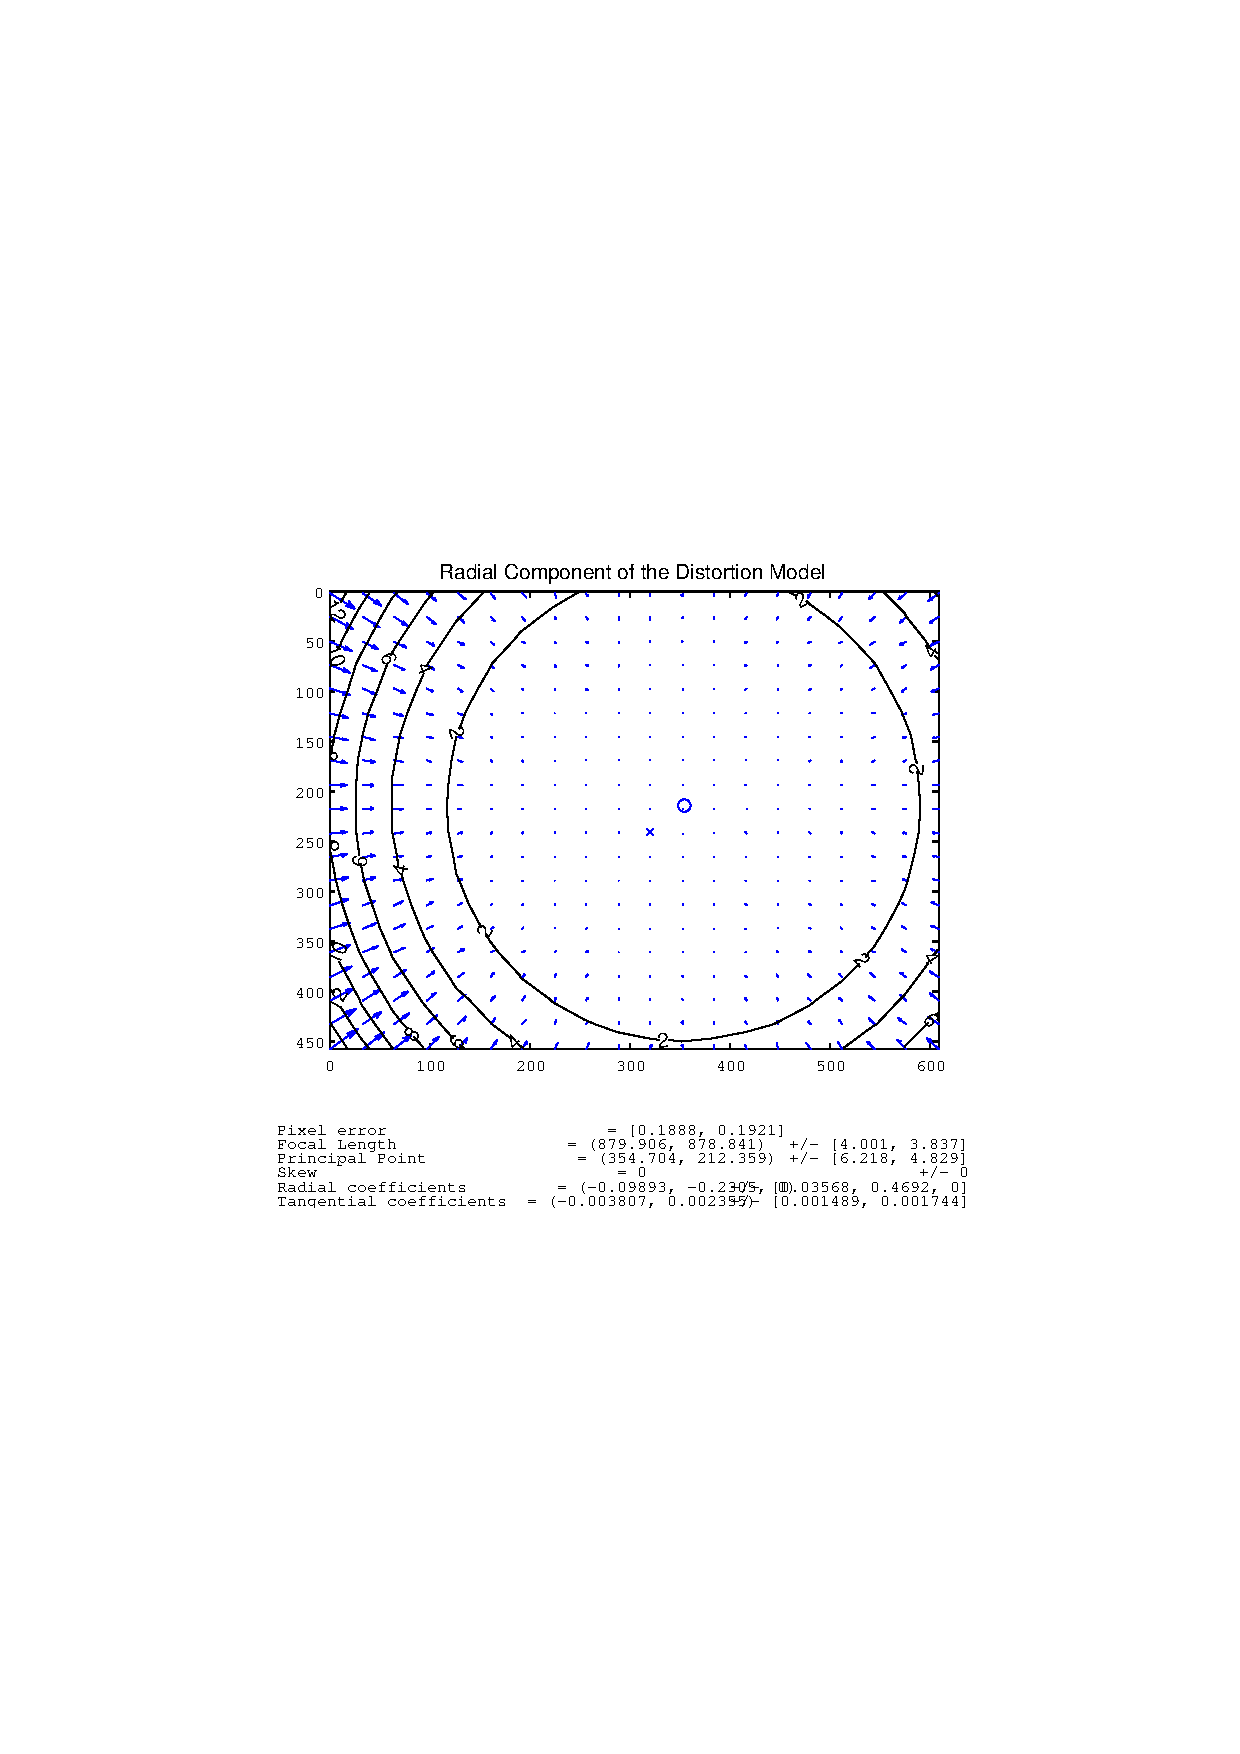
\includegraphics[width=0.45\textwidth]{pics/left_rad_dist}
    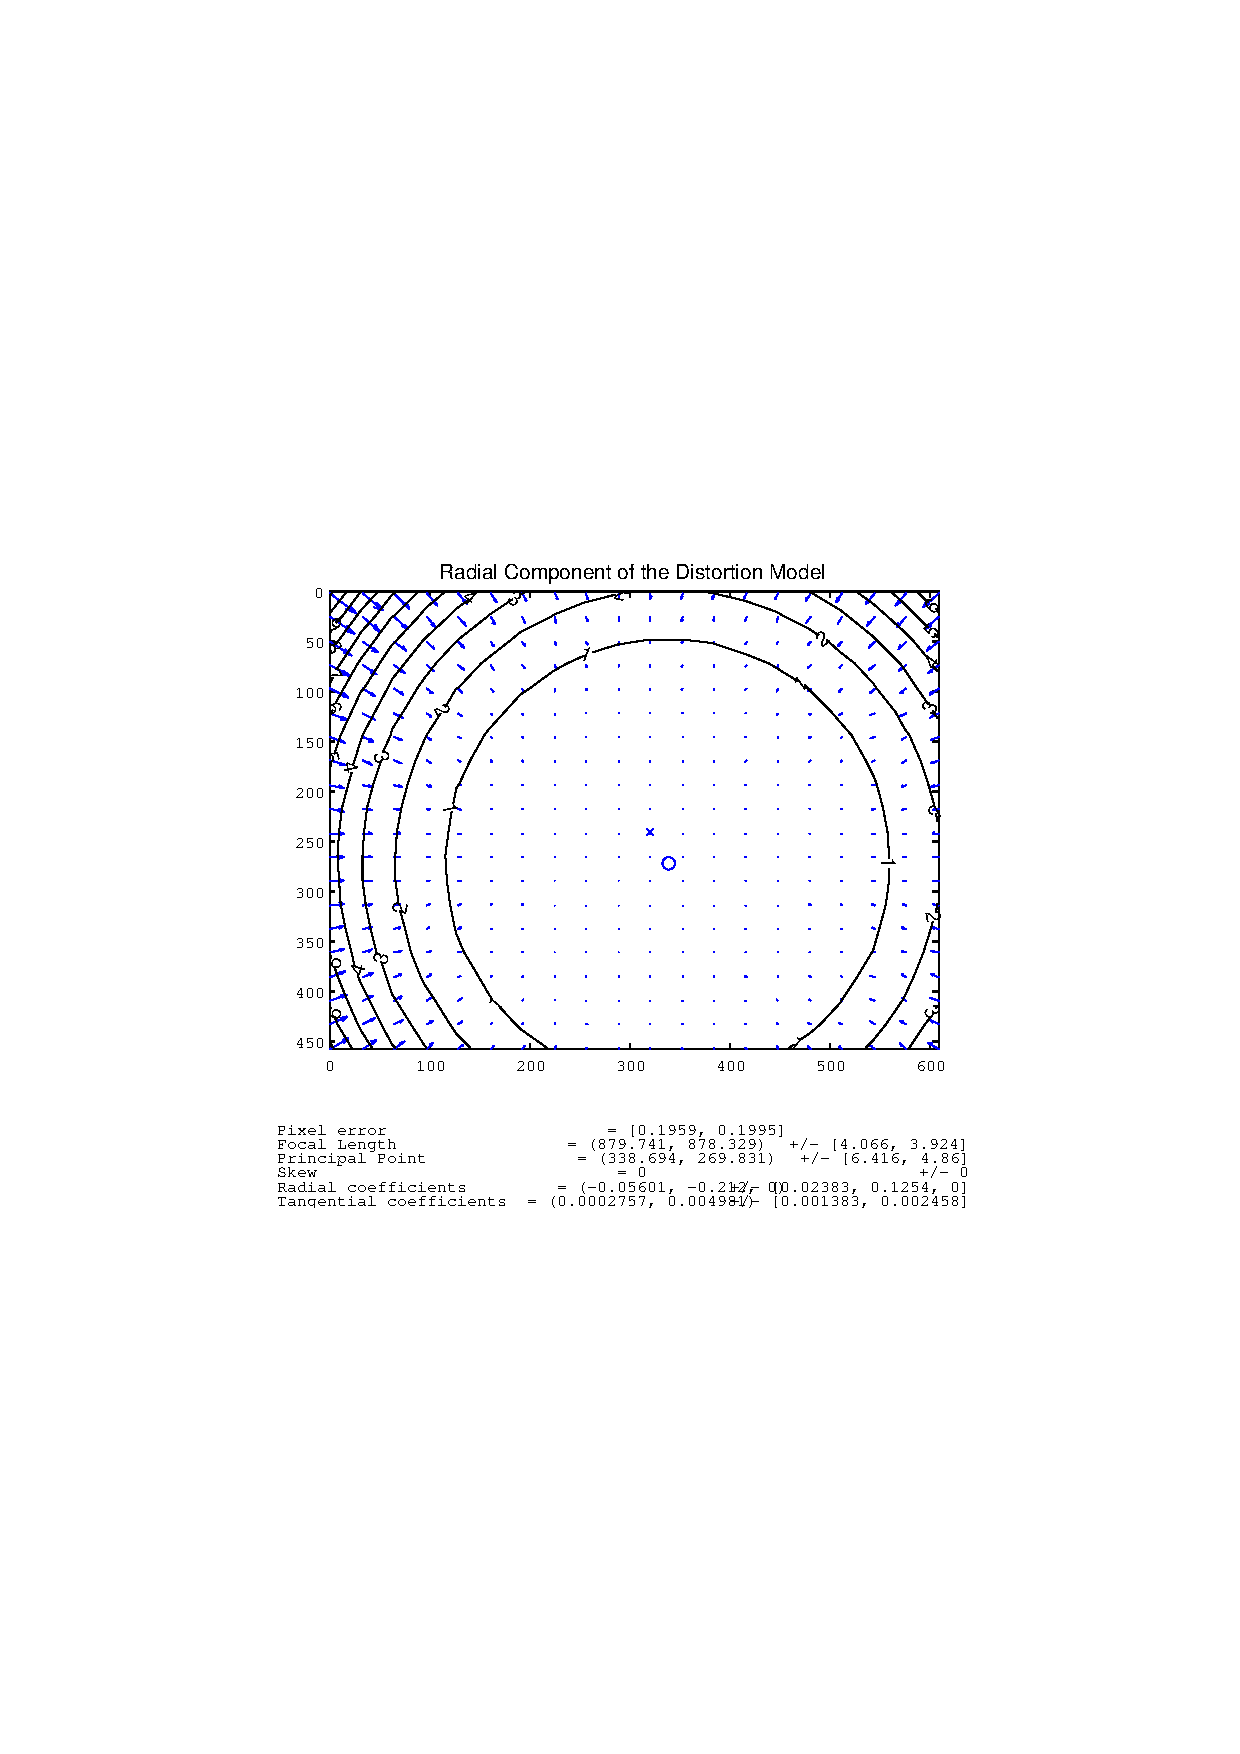
\includegraphics[width=0.45\textwidth]{pics/right_rad_dist}
    \caption{The radial distortions of the left and right camera of the stereo rig}
    \label{chap8:fig-rad-dist}
\end{figure}
The field-of-view of the stereo rig is the incision of the two images. 

Another limit of the cameras, besides the field-of-view is the light sensitivity and
the amount of noise on the captured images. The amount of noise in the captured pictures
are dependant on the portion of ambient light in the scene. In the tests no extra
light source where used, only ambient and sunlight from the surroundings. This was because
the pipe bends where turned towards the window which gave much sunlight. If a artificial
light source were included in the tests, some of the features would be sharper and the
matching would have produced better results. 




\section{Why did it perform this way?}



